\documentclass{article}
\usepackage{titling}
\usepackage{graphicx}
\usepackage{caption}
\usepackage{helvet}
\usepackage{hyperref}
\usepackage{sectsty}

% Define font size and family for sections
\sectionfont{\fontsize{10}{12}\selectfont\renewcommand{\familydefault}{\sfdefault}}
\subsectionfont{\fontsize{10}{12}\selectfont\renewcommand{\familydefault}{\sfdefault}}
\subsubsectionfont{\fontsize{10}{12}\selectfont\renewcommand{\familydefault}{\sfdefault}}
\paragraphfont{\fontsize{10}{12}\selectfont\renewcommand{\familydefault}{\sfdefault}}
\subparagraphfont{\fontsize{10}{12}\selectfont\renewcommand{\familydefault}{\sfdefault}}
\renewcommand{\familydefault}{\rmdefault} % Reset default to Roman for title page

\title{Relazione progetto Programmazione ad Oggetti}
\author{Alberto Canavese\\Numero matricola: 2076423}
\date{A.A. 2023/24}

\begin{document}
    % Pagina titolo
    \pretitle{\begin{center}\LARGE}
    \posttitle{\end{center}}
    \preauthor{\begin{center}\large \lineskip 0.5em}
    \postauthor{\end{center}}
    \predate{\begin{center}\large}
    \postdate{\end{center}}
    \maketitle

    % Change font and size for the rest of the document
    \renewcommand{\familydefault}{\sfdefault} % Set default to sans serif
    \fontsize{10}{12}\selectfont

    % Pagina introduzione
    \newpage
    \section{Introduzione}
    \textbf{Sensor Hub} è un'applicazione realizzata con Qt Creator che consente di gestire tre tipi
    diversi di sensori virtuali: \textbf{humidity\_sensor}, \textbf{dust\_sensor} e \textbf{temperature\_sensor}.
    
    Il programma permette di creare, modificare, cancellare e ricercare i sensori tramite un'interfaccia
    grafica intuitiva.
        
    Vi sono due modi per dichiarare un sensore:
    \begin{itemize}
        \item \textbf{Tramite interfaccia}: Creando da zero un sensore con i dati inseriti dall'utente tramite un'opportuna finestra di dialogo.
        \item \textbf{Tramite file}: Importando, tramite finestra di dialogo, un file txt contenente i dati del sensore.
    \end{itemize} 
    La funzionalità principale di \textbf{Sensor Hub} è la possibilità di avviare una simulazione di lettura dati per un qualsiasi sensore selezionato. 
    
    La simulazione genera una serie di dati, coerenti con il tipo di sensore, che vengono visualizzati graficamente utilizzando la classe \textbf{Qt Charts}.

    Tutti i dati di simulazione e tutti i dettagli di ogni sensore vengono salvati nel medesimo file di testo, in modo da supportare la persistenza dei dati. 

    Infine, è anche possibile esportare tutti i sopracitati dati sotto forma di file \textbf{.txt} tramite un context menu.

    \section{Descrizione del modello}
    Il modello logico è composto da una gerarchia di classi che rappresenta i vari tipi di sensori istanziabili e simulabili. 
        
    Di seguito il diagramma UML:    
    \begin{figure}[h!]
        \centering
        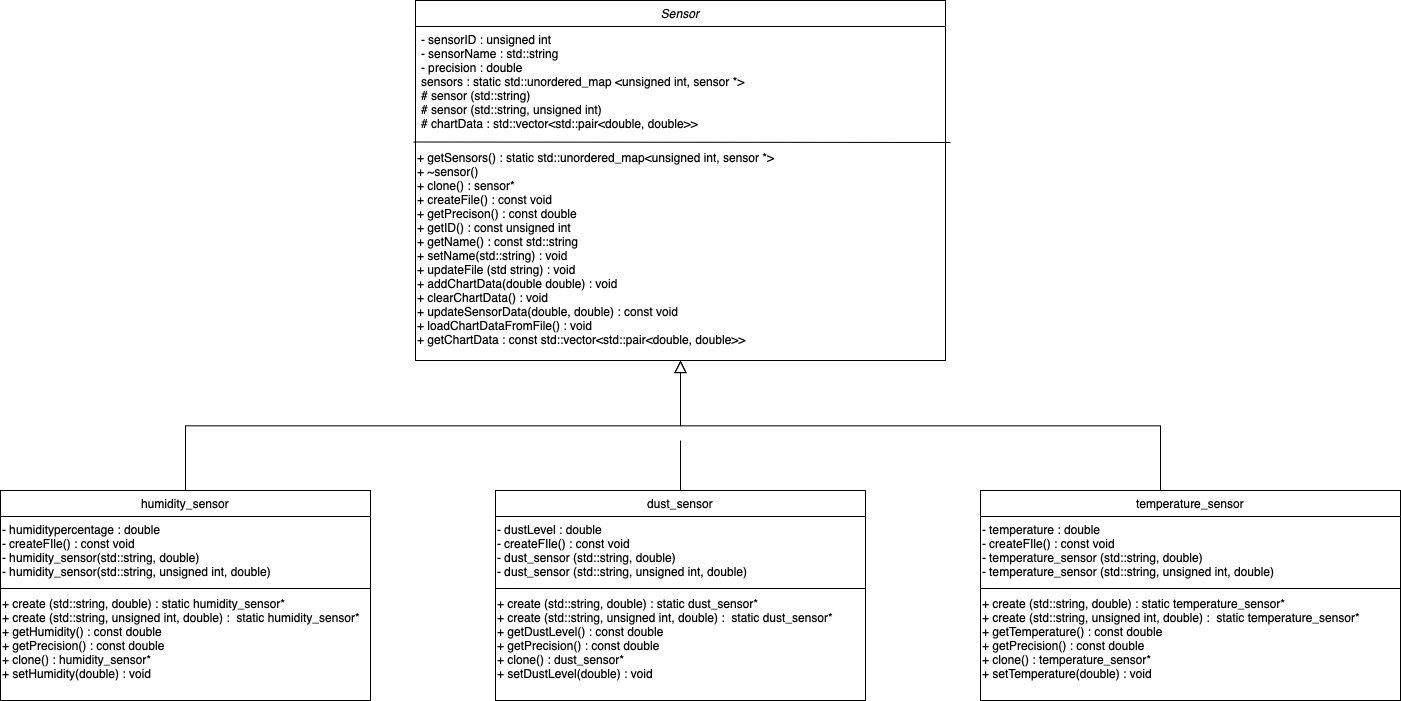
\includegraphics[width=0.8\textwidth]{UML.png}
        \caption*{Diagramma UML}
    \end{figure}

    \newpage
    \noindent Il modello parte da una classe astratta \textbf{“sensor”} che contiene le informazioni comuni a tutti i tipi di sensori, quali: \textbf{ID}, \textbf{nome} e \textbf{precisione}.
    Per entrambi gli attributi comuni sono stati implementati dei metodi getter e nel caso del nome è stato implementato il rispettivo metodo setter per permettere la modifica del nome del sensore anche dopo l’istanziazione. 

    \noindent La classe astratta, implementa una struttura dati di tipo \textbf{std::unordered\_map} che memorizza coppie di dati ID + puntatore a sensore, in modo da tenere traccia di tutti gli ID già in uso e di evitare doppioni.

    \noindent Sono inoltre presenti metodi concreti, comuni a tutti i tipi di sensori, che permettono la gestione della simulazione, garantendo la persistenza dei dati, i metodi sono:
    \textbf{addChartData()}, \textbf{clearChartData()}, \textbf{updateSensorData()} e \textbf{loadChartDataFromFile()}.

    \noindent Infine sono presenti dei metodi virtuali puri, in quanto la loro implementazione e funzione varia in base al tipo di sensore, questi metodi sono: \textbf{clone()} e \textbf{createFile()}.

    Le sottoclassi rappresentano tre tipi diversi di sensori: \textbf{humidity\_sensor}, \textbf{dust\_sensor} e \textbf{temperature\_sensor},  ciascuna di queste tre classi offre la sua implementazione del metodo createFile().

    \noindent In particolare i dati contenuti all’interno del file di testo varieranno in base al tipo di sensore, in modo da permettere a sensor\_hub di riconoscere che tipo di sensore istanziare nel caso venga importato e non creato direttamente all’interno del programma tramite interfaccia grafica. 

    \section{Polimorfismo}
    Nello sviluppo di questo progetto, l'utilizzo del polimorfismo riguarda la gerarchia delle classi derivate dalla classe base “sensor”.   


    Il polimorfismo viene impiegato per diverse funzionalità, come: la clonazione degli oggetti, la gestione dei dati specifici di ciascun sensore e la creazione di file che contengono le informazioni di un determinato sensore.

    \noindent La classe \textbf{sensor} dichiara diversi metodi virtuali puri che devono essere implementati dalle classi derivate,  tra questi, i metodi \textbf{clone} e \textbf{createFile} sono particolarmente importanti:

    \noindent Il metodo \textbf{clone} è utilizzato per realizzare il design pattern Clone, permettendo la creazione di copie polimorfe degli oggetti senza conoscere il loro tipo concreto al momento della clonazione. 

    \noindent Il metodo \textbf{createFile}, anch'esso dichiarato virtuale puro nella classe sensor, è implementato da tutte le classi derivate per creare file che contengono i dati specifici di ciascun tipo di sensore.   Questo metodo permette di gestire la persistenza dei dati in maniera polimorfica, in modo che il codice chiamante possa invocare createFile su un puntatore di tipo sensor senza preoccuparsi del tipo concreto dell'oggetto a cui si riferisce.


    \noindent Oltre a questi metodi, la classe sensor fornisce anche metodi virtuali non puri come \textbf{updateSensorData} e \textbf{loadChartDataFromFile}, che possono essere sovrascritti dalle classi derivate per fornire comportamenti specifici.


    \noindent Vi è anche un utilizzo del polimorfismo di minor rilevanza, dovuto alla necessità di avere un “costruttore di copia polimorfo”, che viene realizzato tramite il design pattern Clone come descritto sopra.  

    \noindent Le classi dust\_sensor, humidity\_sensor e temperature\_sensor dichiarano e implementano i metodi clone e createFile, garantendo che ogni tipo di sensore possa essere duplicato e salvato correttamente.


    In conclusione, il polimorfismo nel programma consente di gestire in maniera flessibile e estendibile le operazioni comuni sui sensori, come la clonazione e la creazione di file, delegando alle classi derivate la responsabilità di definire i dettagli specifici di ciascun tipo di oggetto.   Questo approccio facilita l'aggiunta di nuovi tipi di sensori in futuro, senza necessità di modifiche radicali al codice esistente.

    \section{Persistenza dei dati}
    Per implementare la persistenza dei dati vengono utilizzati dei semplici file .txt.
    Per ogni sensore istanziato viene creato automaticamente un file di testo contenente tutti i suoi dettegli. 

    \noindent Inoltre, nel file di testo, dopo tutti i dettagli viene aggiunta una voce "\textbf{chart data:}" che contiene tutte le informazioni generate durante la simulazione di un determinato sensore.

    \noindent Quindi, quando viene esportato un file di un sensore sono anche presenti tutte le informazioni di un eventuale simulazione passata.

    \noindent Viceversa, se un sensore viene importato da file di testo vengono riconosciuti i dati relativi all’ultima simulazione e il grafico relativo a quest’ultima viene generato sulla base di questi valori e mostrato all’utente.

    \section{Funzionalità implementate}
    \textbf{sensor\_hub} implementa le seguenti funzionalità:
    \begin{itemize}
        \item Creazione di sensori in-app tramite interfaccia grafica.
        \item Importazione di sensori da file di testo tramite interfaccia grafica.
        \item Possibilità di modificare il nome di un sensore tramite interfaccia grafica.
        \item Possibilità di cancellare tutti i dati relativi a un sensore tramite interfaccia grafica.
        \item Possibilità di cercare un sensore tramite nome o ID grazie a una casella di testo.
        \item Possibilità di avviare e di terminare simulazioni di letture dati di tutti i tipi di sensori.
        \item Gestione nel caso si cerchi di istanziare due sensori con lo stesso ID.
    \end{itemize}
    \newpage Le funzionalità grafiche, invece, sono le seguenti:
    \begin{itemize}
        \item Elenco laterale nel quale vengono mostrati tutti i sensori istanziati.
        \item Bottone “+” che permette di creare un nuovo sensore, una volta premuto verrà chiesto se il sensore si vuole creare da 0, oppure importare un file di testo.
        \item Bottone “-“ che permette di rimuovere il sensore selezionato dal programma, il che comporta anche l’eliminazione del file di testo dall’apposita cartella. 
        \item Bottoni per iniziare o terminare una simulazione: posizionati in basso nella schermata principale vi sono due bottoni che permettono di iniziare/terminare una simulazione per il sensore selezionato.
        \item Grafico posizionato al centro della schermata che permette di visualizzare in tempo reale una rappresentazione della simulazione in corso.
        \item Immagini rappresentative per tipo di sensore: ogni tipo di sensore è associato ad un immagine significativa che viene mostrata nella lista dei sensor e ne rappresenta la tipologia.
        \item Label che mostra i dettagli del sensore selezionato dalla barra laterale.
    \end{itemize}

    \section{Rendicontazione ore} 

    \begin{table}[!ht]
        \centering
        \begin{tabular}{|l|l|l|}
        \hline
            \textbf{Attività} & \textbf{Ore Previste} & \textbf{Ore Effettive} \\ \hline
            Studio e progettazione & 10 & 10 \\ \hline
            Sviluppo Del Codice Del Modello & 10 & 11 \\ \hline
            Studio Del Framework Qt & 10 & 12 \\ \hline
            Sviluppo Del Codice Della GUI & 10 & 15 \\ \hline
            Ricerca E Editing Degli Assets & 1 & 1 \\ \hline
            Test E Debug & 5 & 7 \\ \hline
            Stesura Della Relazione & 4 & 4 \\ \hline
            \textbf{TOTALE} & 50 & 60 \\ \hline
        \end{tabular}
    \end{table}
    Il monte ore è stato superato principalmente per tre motivi:
    \begin{itemize}
        \item La necessità di approfondire il framework Qt.
        \item Problemi riscontrati con l'IDE Qt Creator per quanto riguarda l'utilizzo della libreria QtCharts.
        \item Debug: ho riscontrato alcune difficoltà nel correggere alcuni malfunzionamenti generali. 
    \end{itemize}
    
\end{document}
